\documentclass[11pt,letterpaper]{article}
\usepackage[left=.80in,right=.80in,top=.76in,bottom=.72in,headheight=15pt,headsep=15pt,footskip=22pt]{geometry}
\usepackage[T1]{fontenc}
\usepackage{lmodern,microtype,amsmath,amssymb,mathtools}
\usepackage{graphicx,array,booktabs,tabularx,multicol}
\usepackage[table]{xcolor}
\usepackage{tikz,tcolorbox,fancyhdr}
\usetikzlibrary{arrows.meta,decorations.pathreplacing,patterns,calc}
\usepackage[hidelinks,pdfauthor={Komorebi P.},pdftitle={Paper XII: A Visual Appendix},pdfsubject={Worked examples for completed local conditions, support, Fitting strata, Hecke packets and conditional automorphic completion}]{hyperref}
\usepackage{bookmark}
\renewcommand*{\HyperDestNameFilter}[1]{VA.#1}
\setlength{\parindent}{0pt}
\setlength{\parskip}{6pt}
\setlength{\emergencystretch}{2em}
\renewcommand{\arraystretch}{1.2}
\linespread{1.04}
\setlength{\abovedisplayskip}{7pt}
\setlength{\belowdisplayskip}{7pt}
\pagestyle{fancy}\fancyhf{}
\fancyhead[L]{\sffamily\fontsize{8}{10}\selectfont PAPER XII\quad /\quad VISUAL APPENDIX}
\fancyhead[R]{\sffamily\fontsize{8}{10}\selectfont KOMOREBI P.}
\fancyfoot[L]{\sffamily\fontsize{8}{10}\selectfont Reader's edition\quad\textbullet\quad Formal source: v0.17.0}
\fancyfoot[R]{\sffamily\small V\,--\,\thepage}
\renewcommand{\headrulewidth}{.35pt}\renewcommand{\footrulewidth}{0pt}
\newcommand{\OO}{\mathcal O}
\newcommand{\FF}{\mathbb F}\newcommand{\QQ}{\mathbb Q}\newcommand{\ZZ}{\mathbb Z}\newcommand{\RR}{\mathbb R}
\newcommand{\Spec}{\operatorname{Spec}}\newcommand{\Supp}{\operatorname{Supp}}\newcommand{\Fitt}{\operatorname{Fitt}}
\newcommand{\Ann}{\operatorname{Ann}}\newcommand{\coker}{\operatorname{coker}}\newcommand{\im}{\operatorname{im}}
\newcommand{\rank}{\operatorname{rank}}\newcommand{\Tr}{\operatorname{Tr}}\newcommand{\id}{\operatorname{id}}
\newcommand{\whot}{\mathbin{\widehat\otimes}}\newcommand{\m}{\mathfrak m}\newcommand{\p}{\mathfrak p}
\newcommand{\head}[1]{\par\vspace{4pt}{\sffamily\bfseries\normalsize #1}\par\vspace{1pt}}
\newcommand{\captiontext}[1]{\par\noindent{\footnotesize\color{black!70}#1\par}}
\newtcolorbox{insight}{colback=black!3,colframe=black!55,boxrule=0pt,leftrule=1.1pt,arc=0pt,left=10pt,right=10pt,top=6pt,bottom=6pt,before skip=9pt,after skip=8pt}
\newcommand{\takeaway}[1]{\begin{insight}\textbf{Read this as:}\ #1\end{insight}}
\newcommand{\vfig}[2][.92]{\begin{center}\resizebox{#1\linewidth}{!}{\input{graphics/#2.tex}}\end{center}}
\newcolumntype{Y}{>{\raggedright\arraybackslash}X}
\newif\ifstarted\startedfalse
\newcommand{\vpage}[4]{\ifstarted\clearpage\else\startedtrue\fi
\phantomsection\label{v:#1}\pdfbookmark[1]{V#1. #2}{visual#1}
{\sffamily\fontsize{9}{11}\selectfont\bfseries #3\par}\vspace{5pt}
{\sffamily\bfseries\fontsize{24}{27}\selectfont #2\par}\vspace{5pt}
{\sffamily\fontsize{8.7}{11}\selectfont\color{black!65} #4\par}\vspace{10pt}}
\newcommand{\pagerefV}[1]{\hyperref[v:#1]{V\,--\,#1}}
\begin{document}
% ---------------------------------------------------------------------------
\vpage{1}{Seeing the objects}{A READER'S COMPANION}{Patching Support, Hecke Packets, and Conditional Automorphic Completion}
The paper repeatedly asks three different questions: does an object exist, where is a supplied object nonzero, and when does that object have the desired arithmetic meaning? This appendix makes those distinctions tangible through examples that can be followed by hand.

\begin{insight}
\begin{tabularx}{\linewidth}{@{}p{.18\linewidth}Y@{}}
\textbf{Existence} & Is there a represented deformation problem, a nonzero carrier, or a compatible family to start with?\\[3pt]
\textbf{Support} & At which prime ideals does the supplied module or complex survive?\\[3pt]
\textbf{Realization} & Does the surviving eigensystem come from a classical automorphic object with the required attached representation?
\end{tabularx}
\end{insight}

\head{Three models, rather than one overloaded analogy}
\begin{tabularx}{\linewidth}{@{}p{.20\linewidth}Y>{\raggedright\arraybackslash}p{.15\linewidth}@{}}\toprule
\textbf{Model} & \textbf{What it lets you see} & \textbf{Pages}\\\midrule
A formal thickening & Conditions on power series, infinitesimal points, obstructed lifts, and compatible precision levels. & \pagerefV{3}--\pagerefV{5}\\
A presented module & Matrix rank, support, Fitting ideals, changes of coordinates, and nonreduced structure. & \pagerefV{6}--\pagerefV{8}\\
A finite Artin algebra & Generalized eigenspaces, nilpotent directions, canonical packets, and empty packet modules. & \pagerefV{12}--\pagerefV{14}\\\bottomrule
\end{tabularx}

The models are connected by the paper's theorems, but they are not the same ring. A polynomial coordinate plane is not a complete local spectrum, and a local branch is not an Artin product factor. Explicitly changing models prevents a picture from silently changing the hypotheses.

\head{A route through the appendix}
Use the object atlas on \pagerefV{2} when a symbol becomes unfamiliar. The local model starts on \pagerefV{3}; the matrix model on \pagerefV{6}. Pages \pagerefV{9}--\pagerefV{11} explain what quotients, patching, and derived fibers preserve. Pages \pagerefV{15}--\pagerefV{16} separate finite occupancy from genuine infinite compatibility. The exact arithmetic boundary is on \pagerefV{17}.

\head{How to read a visual claim}
Each page gives an explicit object, a calculation, and a source reference. Coordinate sketches display only the stated real points. Coefficient arrays and finite specialization diagrams describe the stated algebraic data exactly. Line thickness never stands for nilpotent multiplicity.

\takeaway{These are explanations of the formal release, not additional assumptions or new Lean certificates. The accompanying scripts check the explicit finite calculations. They do not establish universal arithmetic existence.}

% ---------------------------------------------------------------------------
\vpage{2}{An atlas of the objects}{ORIENTATION}{Main text: Sections 2, 3, 6, 7, 8 and 12}
A \emph{ring} describes possible points. A \emph{module over the ring} describes what is carried at those points. A nonempty space of possibilities does not imply a nonzero carrier at every point.

{\small
\begin{tabularx}{\linewidth}{@{}p{.20\linewidth}Yp{.22\linewidth}@{}}\toprule
\textbf{Symbol} & \textbf{Object and role} & \textbf{Keep separate}\\\midrule
$\OO,\ k$ & Complete coefficient ring and its residue field. The formal teaching model uses $\OO=\ZZ_5$, $k=\FF_5$. & Coefficients versus variables.\\
$R_i,\ I_i$ & A supplied local ring and the ideal imposing a declared local condition. & A quotient condition is not an idempotent.\\
$R^{\mathrm{loc}}$ & Completed tensor product of the local rings over $\OO$. & Completion uses the declared adic topology.\\
$J$ & Closed ideal generated by the images of all $I_i$ in $R^{\mathrm{loc}}$. & Closure, not just a finite list of tests.\\
$R^{\mathrm{loc},\tau}$ & Completed tensor of the local quotients; identified with $R^{\mathrm{loc}}/J$. & A constructed comparison, not assumed notation.\\
$R^\square$ & Supplied global ring receiving the local structural maps. & Representability is arithmetic input.\\
$R^\tau$ & Completed global base change imposing the simultaneous local conditions. & Does not create a missing residual point.\\
$R_\infty,\ M_\infty$ & Patched ring and its module; a perfect complex is used in the derived version. & Freeness over an auxiliary ring is weaker than full support.\\
$R,\ M$ & Finite-level ring and carrier after the specified quotient and control isomorphism. & The module may be zero on a component.\\
$T,\ H$ & Hecke algebra and its ordinary or derived carrier. & Ring comparison does not imply classicality.\\
$e_{\m}H$ & Packet selected by a canonical Artin idempotent. & A generalized packet need not be an eigenspace.\\
$Y_m$ & Stable image at level $m$ of an inverse system. & Nonzero levels alone do not give a nonzero limit.\\\bottomrule
\end{tabularx}}

\head{Why arrows reverse when points appear}
A ring map $f:R\to T$ sends a prime of $T$ to its inverse image in $R$:
\[
f^*:\Spec T\longrightarrow\Spec R,\qquad \mathfrak q\longmapsto f^{-1}(\mathfrak q).
\]
Similarly, a point $y:T\to E'$ gives the point $y\circ f:R\to E'$. The equality $y\circ f=x$ is an actual requirement in the final theorem, not a consequence of drawing a connecting arrow.

% ---------------------------------------------------------------------------
\vpage{3}{Local conditions remove directions}{MODEL A / A FORMAL THICKENING}{Main text: Theorem 3.1 and Corollary 3.2}
Fix $\OO=\ZZ_5$. Take two independent local variables and impose two different kinds of condition:
\[
R_1=\OO[[x]],\quad I_1=(x^2),\qquad
R_2=\OO[[y]],\quad I_2=(y).
\]
Their completed local tensor is $A=\OO[[x,y]]$. The closed generated ideal is $J=(x^2,y)$, and both routes through Theorem 3.1 give
\[
(R_1/I_1)\whot_{\OO}(R_2/I_2)
\cong A/J
\cong \OO[\varepsilon]/(\varepsilon^2).
\]

\vfig[.96]{monomial_quotient}
\captiontext{An exact finite window of monomials over $\OO$. Crosses mean that the monomial is zero in the quotient; they do not represent a small numerical coefficient. All terms outside the window satisfy the same divisibility rule.}

\head{The calculation behind the image}
For $f=\sum_{i,j\ge0}a_{ij}x^iy^j$, reduction gives
\[
f\longmapsto a_{00}+a_{10}\varepsilon.
\]
Every term involving $y$ vanishes. Every term involving $x^2$ vanishes. The class of $x$ does \emph{not} vanish: it becomes a nonzero element whose square is zero. The quotient is a free $\OO$-module with basis $1,\varepsilon$.

\head{Why a point picture alone would miss this}
After passing to the special fiber, $k[\varepsilon]/(\varepsilon^2)$ has the same underlying one-point spectrum as $k$. The extra direction is visible in the algebra and in maps from test rings, not as a second point. It is also not a second component or a second Artin packet.

\takeaway{The condition $y=0$ deletes a variable. The condition $x^2=0$ retains a first-order nilpotent direction. Both are quotient conditions, but their effects are different.}

% ---------------------------------------------------------------------------
\vpage{4}{A point is a test of the equations}{MODEL A / FACTORIZATION AND OBSTRUCTION}{Main text: Proposition 3.3; this explicit example also exhibits a failed infinitesimal lift}
Let $R^\square=\OO[[u,v]]$ and send $x\mapsto u$, $y\mapsto v-u$. The local conditions become
\[
u^2=0,\qquad v-u=0,
\quad\text{so}\quad
R^\tau=\OO[[u,v]]/(u^2,v-u)\cong\OO[\varepsilon]/(\varepsilon^2).
\]
Probe this ring using $D_3=\FF_5[\delta]/(\delta^3)$, with the fixed coefficient map $\ZZ_5\to\FF_5$. A continuous local point is specified by
\[
u\longmapsto a\delta+b\delta^2,\qquad
v\longmapsto c\delta+d\delta^2,
\qquad a,b,c,d\in\FF_5.
\]
It factors through $R^\tau$ precisely when
\[
a^2=0,\quad c=a,\quad d=b
\quad\Longleftrightarrow\quad a=c=0,\ d=b.
\]

\begin{minipage}[t]{.48\linewidth}\centering
{\sffamily\small\bfseries First-order coefficients}\par
\vfig[.68]{points_slopes}
\captiontext{Only the slope pair $(a,c)=(0,0)$ survives. Each square initially has 25 choices of $(b,d)$.}
\end{minipage}\hfill
\begin{minipage}[t]{.48\linewidth}\centering
{\sffamily\small\bfseries Remaining second-order coefficients}\par
\vfig[.68]{points_curvatures}
\captiontext{Once $a=c=0$, the five diagonal choices $d=b$ give all accepted points.}
\end{minipage}

\head{An obstruction you can calculate}
There are $5^4=625$ candidate $D_3$-points and exactly five accepted points. Over $D_2=\FF_5[\delta]/(\delta^2)$, however, the five maps $u=v=a\delta$ all satisfy the equations. Reduction of \emph{every} accepted $D_3$-point gives the zero $D_2$-point. The four nonzero tangent directions therefore do not lift to order three.

\takeaway{A point satisfies equations in a target ring. A tangent direction can exist while its next-order lift fails. The factorization theorem identifies the condition; it does not promise that every point lifts.}

% ---------------------------------------------------------------------------
\vpage{5}{Completion retains every precision}{MODEL A / COMPATIBLE COEFFICIENTS}{Main text: Theorem 3.1; reconstruction and finite occupancy in Section 10}
For $B=\ZZ_5[\varepsilon]/(\varepsilon^2)$, consider the finite quotient rings
\[
B_n=(\ZZ/5^n\ZZ)[\varepsilon]/(\varepsilon^2),
\qquad |B_n|=5^{2n},\qquad B\cong\varprojlim_n B_n.
\]
A point of the limit is a \emph{single compatible choice} at every level, not unrelated choices from the nonempty finite rings.

\head{Two explicit 5-adic numbers}
Choose the canonical digits
\[
\alpha_j=(j^2+1)\bmod5,\qquad \beta_j=(2j+1)\bmod5,
\]
with values in $\{0,1,2,3,4\}$. Set $a=\sum_{j\ge0}\alpha_j5^j$ and $b=\sum_{j\ge0}\beta_j5^j$. The element $a+\varepsilon b$ is determined by the following coefficient array.

\vfig[.87]{adic_digits}
\captiontext{Cutting before column $5^n$ produces reduction modulo $5^n$. The digit formulas define every column, including those not drawn.}

\begin{center}\small
\begin{tabular}{@{}lrrrrr@{}}\toprule
$n$ & 1 & 2 & 3 & 4 & 5\\\midrule
$5^n$ & 5 & 25 & 125 & 625 & 3125\\
$a\bmod5^n$ & 1 & 11 & 11 & 11 & 1261\\
$b\bmod5^n$ & 1 & 16 & 16 & 266 & 2766\\\bottomrule
\end{tabular}
\end{center}
Every longer prefix reduces to the previous one; the digit formulas specify all later coefficients.

\head{Where the topology enters}
The $5$-adic and $(5,\varepsilon)$-adic topologies on $B$ agree: for every $n$,
\[
(5,\varepsilon)^{n+1}\subseteq 5^nB\subseteq(5,\varepsilon)^n.
\]
For the general quotient theorem, the condition ideal must be closed. A continuous map to a Hausdorff target has closed kernel: vanishing on the original generators therefore kills their closure.



% ---------------------------------------------------------------------------
\vpage{6}{A matrix becomes a support locus}{MODEL B / FITTING STRATA}{Main text: Theorems 6.2, 6.3 and 6.4}
Now change models. Let $R=k[x,y]$ for a field $k$, and present a module by
\[
R^2\xrightarrow{A}R^2\longrightarrow M\longrightarrow0,
\qquad
A=\begin{pmatrix}x&0\\0&y\end{pmatrix}.
\]
The relations are $xe_1=0$ and $ye_2=0$, so $M\cong R/(x)\oplus R/(y)$.

\begin{minipage}[c]{.48\linewidth}
\vfig[.98]{support_axes}
\end{minipage}\hfill
\begin{minipage}[c]{.48\linewidth}
{\sffamily\bfseries The minor calculation}\par
\[
\begin{aligned}
\Fitt_0(M)&=(xy),\\
\Fitt_1(M)&=(x,y),\\
\Fitt_j(M)&=R\quad(j\ge2).
\end{aligned}
\]
At a prime $\p$, reduce the matrix to its residue field:
\[
\mu_{\p}(M)=2-\rank A(\p).
\]
Two independent relations disappear at the origin. Only one disappears along either punctured axis.
\end{minipage}
\captiontext{For the drawing, take $k=\RR$. It shows real closed points, not every point of $\Spec R$. The displayed ideals and rank criterion describe the full algebraic loci over any field.}

\begin{center}\small
\begin{tabular}{@{}llll@{}}\toprule
Position & Matrix rank & Fiber dimension & What survives\\\midrule
$x\ne0$, $y\ne0$ & 2 & 0 & neither generator\\
$x=0$, $y\ne0$ & 1 & 1 & the $e_1$ direction\\
$x\ne0$, $y=0$ & 1 & 1 & the $e_2$ direction\\
$x=y=0$ & 0 & 2 & both directions\\\bottomrule
\end{tabular}
\end{center}
Thus $\Supp(M)=V(xy)=V(x)\cup V(y)$, whereas the locus where the fiber needs at least two generators is $V(x,y)$. The latter is a \emph{higher} Fitting stratum.

\takeaway{Support asks whether any direction survives. Higher Fitting strata ask how many generators the residue-field fiber needs. This is not an automorphic multiplicity formula.}

% ---------------------------------------------------------------------------
\vpage{7}{The same support can hide more algebra}{MODEL B / NILPOTENT STRUCTURE}{Main text: Theorems 6.3--6.4; distinguish an ideal from its vanishing set}
Compare the previous module with a slightly different presentation:
\[
M=\coker\begin{pmatrix}x&0\\0&y\end{pmatrix},
\qquad
M'=\coker\begin{pmatrix}x^2&0\\0&y\end{pmatrix}.
\]
Their support sets coincide. Their residue-field fiber dimensions also coincide at every prime. But their Fitting ideals do not.

\begin{center}
\begin{tabular}{@{}lll@{}}\toprule
 & $M$ & $M'$\\\midrule
Zeroth Fitting ideal & $(xy)$ & $(x^2y)$\\
First Fitting ideal & $(x,y)$ & $(x^2,y)$\\
Support as a set & $V(x)\cup V(y)$ & $V(x)\cup V(y)$\\
Fiber dimension at $(x,y)$ & 2 & 2\\\bottomrule
\end{tabular}
\end{center}

\head{Magnify transversely, rather than draw a thicker line}
Take the slice $y=1$. The second summand vanishes because $y$ becomes a unit. What remains is
\[
M|_{y=1}\cong k[x]/(x),\qquad
M'|_{y=1}\cong k[x]/(x^2).
\]
The first has basis $1$; the second has basis $1,x$. Multiplication by $x$ distinguishes them exactly:

\begin{center}
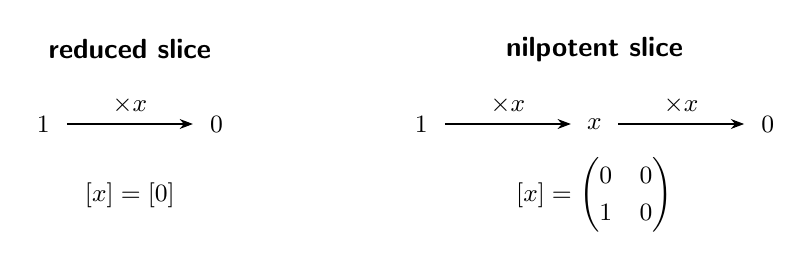
\begin{tikzpicture}[x=1cm,y=1cm,font=\small,>=Stealth]
\node[font=\sffamily\bfseries] at (1.3,1.8) {reduced slice};
\node at (.2,.85) {$1$};\node at (2.4,.85) {$0$};
\draw[->] (.5,.85)--(2.1,.85) node[midway,above] {$\times x$};
\node[font=\sffamily\bfseries] at (7.2,1.8) {nilpotent slice};
\node at (5,.85) {$1$};\node at (7.2,.85) {$x$};\node at (9.4,.85) {$0$};
\draw[->] (5.3,.85)--(6.9,.85) node[midway,above] {$\times x$};
\draw[->] (7.5,.85)--(9.1,.85) node[midway,above] {$\times x$};
\node at (1.3,-.05) {$[x]=[0]$};
\node at (7.2,-.05) {$[x]=\begin{pmatrix}0&0\\1&0\end{pmatrix}$};
\end{tikzpicture}
\end{center}

\head{A test ring detects the higher-stratum thickening}
Let $D=k[\delta]/(\delta^2)$ and send $x\mapsto\delta$, $y\mapsto0$. The ideal $(x^2,y)$ maps to zero, but $(x,y)$ does not. Therefore this $D$-point lies in the scheme defined by the first Fitting ideal of $M'$, but not in the corresponding scheme for $M$.

No extra ordinary point has appeared. What changed is the behavior on nilpotent test rings. This is the same distinction encountered in the formal model on \pagerefV{3}.

\takeaway{Taking $V(I)$ forgets nilpotent thickness. Fitting \emph{ideals} can retain information that both the support set and the fiber-dimension function fail to distinguish.}

% ---------------------------------------------------------------------------
\vpage{8}{Base change is an algebraic pullback}{MODEL B / SPECIALIZATION AND TRANSPORT}{Main text: Proposition 6.5 and Theorem 7.1}
Return to $M=\coker\operatorname{diag}(x,y)$ over $R=k[x,y]$. Pull back along the diagonal $R\to k[t]$, $x\mapsto t$, $y\mapsto t$. The base-changed presentation is literal:
\[
M\otimes_R k[t]\cong\coker\begin{pmatrix}t&0\\0&t\end{pmatrix}
\cong\bigl(k[t]/(t)\bigr)^2.
\]

\begin{minipage}[c]{.44\linewidth}
\vfig[.94]{diagonal_slice}
\end{minipage}\hfill
\begin{minipage}[c]{.51\linewidth}
\head{Both relations vanish together}
\[
(xy)\longmapsto(t^2),\qquad
(x,y)\longmapsto(t).
\]
The support is the origin, but the origin has fiber dimension two. Replacing $(t^2)$ by its radical $(t)$ would lose the zeroth Fitting ideal.

This map is not flat: it is the quotient by $x-y$. The Fitting base-change theorem still applies; it does not require flatness.
\end{minipage}
\captiontext{A real-point shadow of the diagonal slice. The double algebraic contribution is certified by the minor $t^2$, not by the visual thickness of the intersection point.}

\head{An isomorphism changes coordinates, not occupancy}
Over a field of characteristic other than two, the isomorphism
\[
k[x,y]\xrightarrow{\sim}k[a,b],\qquad x\mapsto a+b,\quad y\mapsto a-b
\]
sends the Fitting ideals to $(a^2-b^2)$ and $(a,b)$. The two axes become the two lines $a=b$ and $a=-b$. No previously missing module vector is created by this relabeling.

\head{An extra presentation generator changes nothing}
Replacing $\operatorname{diag}(x,y)$ by $\operatorname{diag}(x,y,1)$ adds a generator killed by the relation $1$. The new maximal minor is $xy$, and the new next-size minors generate $(xy,x,y)=(x,y)$. The module and its intrinsic Fitting ideals are unchanged. This is a small visible instance of the paper's general presentation-independence theorem.

\takeaway{Specialization substitutes into the actual relation matrix. An isomorphism transports all the data. Neither operation may be replaced by an informal edit of the support picture.}

% ---------------------------------------------------------------------------
\vpage{9}{A branch is not an Artin packet}{LOCAL GEOMETRY / AN EXACT FINITE SPECTRUM}{Main text: Proposition 3.4 and Proposition 7.3}
Consider the complete local node
\[
R=k[[x,y]]/(xy),\qquad T=R/(x)\cong k[[y]].
\]
Every prime of $R$ contains $x$ or $y$. Since $k[[x]]$ and $k[[y]]$ are discrete valuation rings, the following diagram lists \emph{all three} prime ideals of $R$ and their specialization relations.

\vfig[.97]{node_spectrum}

\head{What the quotient removes}
As an $R$-module, $T$ has annihilator $(x)$, hence
\[
\Supp_R(T)=V(x)=\{(x),(x,y)\}.
\]
The other generic point $(y)$ is missing because it does not contain $x$. The quotient has not created a disconnected projector summand inside the original local ring. It has changed the ring by imposing an equation.

\head{Why no idempotent selects just this branch}
In a commutative local ring, $e^2=e$ implies $e=0$ or $e=1$. Indeed, $e+(1-e)=1$ forces at least one of $e,1-e$ to be a unit; canceling in $e(1-e)=0$ gives the conclusion. Thus this node has no nontrivial idempotent even though it has two irreducible components.

By contrast, a product of two Artin local rings has two disjoint maximal points, with canonical idempotents $(1,0)$ and $(0,1)$. Those idempotents act on \emph{any supplied module over the product}. Their two ranges are the packets studied on \pagerefV{12}.

\takeaway{Intersecting local components are not product factors. Use quotient ideals and support for the node; use canonical idempotents only where an actual product decomposition exists.}

% ---------------------------------------------------------------------------
\vpage{10}{Free over what? Supported where?}{PATCHING / A COUNTEREXAMPLE WITH A VISIBLE SPECIAL FIBER}{Main text: Theorems 6.7, 6.9 and 6.11; Example 6.13}
Let
\[
S=k[[t]],\qquad R_\infty=S[[x]]/(x(x-t)),\qquad
M_\infty=R_\infty/(x)\cong S.
\]
The module is free of rank one over $S$. Yet over $R_\infty$ its support is only $V(x)$; the generic point $(x-t)$ of the other branch is not occupied.

\begin{minipage}[c]{.47\linewidth}
\vfig[.94]{patching_branches}
\end{minipage}\hfill
\begin{minipage}[c]{.49\linewidth}
\head{Remove the auxiliary variable}
Set $t=0$. Then
\[
R=R_\infty/(t)\cong k[[x]]/(x^2),
\]
\[
M=M_\infty/tM_\infty\cong k.
\]
The two branches meet in a nonreduced special fiber. The relation becomes $x^2=0$, not $x=0$.
\end{minipage}
\captiontext{The drawing is a real algebraic shadow of $x(x-t)=0$. It is not the complete local spectrum. The special fiber's nilpotent structure is recorded by its quotient algebra, not by the point drawn at the intersection.}

\head{Full support need not mean faithful action}
The ring $R$ has one prime, $(x)$. The nonzero module $M=k$ therefore has full support. But $x$ annihilates $M$, so the action is not faithful. It is \emph{nearly faithful}: the annihilator $(x)$ is nilpotent. This distinction disappears over a reduced ring.

\head{The actual descent theorem is one-way}
For a finite module over a Noetherian ring,
\[
\Supp_{R_\infty/(t)}(M_\infty/tM_\infty)
=\Supp_{R_\infty}(M_\infty)\cap V(t).
\]
If the initial support is full, the resulting support is full on the quotient. Our example shows that full support at the quotient can occur even when initial support was not full. It also shows why freeness over $S$ alone is not the required patching hypothesis.

\takeaway{A statement about freeness must name the base ring. A statement about occupancy must name the spectrum. Switching between them without a theorem loses the missing component.}

% ---------------------------------------------------------------------------
\vpage{11}{A vanishing differential changes the fiber}{DERIVED SUPPORT / AN ACTUAL TWO-TERM COMPLEX}{Main text: Definition 6.14 and Theorem 6.16}
Take $R=k[t]$ and the perfect complex
\[
C=\bigl[R\xrightarrow{\;t\;}R\bigr]
\qquad\text{in cohomological degrees }0,1.
\]
Specialization at $t=a$ gives $C_a=[k\xrightarrow{a}k]$. When $a\ne0$, the differential is invertible and the complex is acyclic. When $a=0$, the differential is zero and both cohomology groups survive.

\vfig[.81]{derived_fibers}
\captiontext{A few fibers over $k=\QQ$ are displayed. The statement for every $a\ne0$ follows from invertibility of the scalar $a$; it is not inferred from the sample points.}

\head{Compute before and after specialization}
Before specialization,
\[
H^0(C)=0,\qquad H^1(C)=k[t]/(t).
\]
After \emph{derived} specialization at zero,
\[
C\otimes_R^{\mathbf L}k=[k\xrightarrow{0}k],
\quad H^0\cong k,\quad H^1\cong k.
\]
If one retained only $H^1(C)$ and took its ordinary tensor product with $k$, one would see a single $k$ and miss the extra cohomology in degree zero. The projective complex keeps the information needed for specialization.

\head{The support is still a precise locus}
At any prime not containing $t$, the residue-field differential is invertible. At the prime $(t)$ it is zero. Therefore
\[
\Supp_R(C)=V(t).
\]
Theorem 6.16 identifies support after derived quotient with the intersection of original support and the quotient locus.

\takeaway{Derived nonvanishing means that some cohomology group survives after derived specialization. It neither specifies a classical automorphic class nor eliminates the need for a realization theorem.}

% ---------------------------------------------------------------------------
\vpage{12}{A packet contains an entire Jordan chain}{MODEL C / A NONSEMISIMPLE HECKE ALGEBRA}{Main text: Theorem 8.2, Corollary 8.3 and Example 8.6}
Work over $\QQ$ and let
\[
T=\QQ[z]\big/\bigl((z-1)^2(z+1)^3\bigr),\qquad V=T.
\]
The Chinese remainder theorem gives
\[
T\cong \underbrace{\QQ[\varepsilon]/(\varepsilon^2)}_{T_+,\ z=1+\varepsilon}
\times
\underbrace{\QQ[\eta]/(\eta^3)}_{T_-,\ z=-1+\eta}.
\]
Multiplication by $z$ is an operator $H$. In the ordered local bases $1,\varepsilon$ and $1,\eta,\eta^2$, its matrix is
\[
H=\left(\begin{array}{cc|ccc}
1&0&0&0&0\\1&1&0&0&0\\\hline
0&0&-1&0&0\\0&0&1&-1&0\\0&0&0&1&-1
\end{array}\right).
\]

\vfig[.98]{jordan_packets}
\captiontext{These arrows are the actual nilpotent actions $H-1$ and $H+1$. Each nonzero displayed basis vector belongs to the indicated packet. Only the last nonzero vector in each chain is an ordinary eigenvector.}

\head{The projectors can be written explicitly}
Modulo $(z-1)^2(z+1)^3$, put
\[
e_+(z)=\frac{(5-3z)(z+1)^3}{16},\qquad e_-(z)=1-e_+(z).
\]
Then $e_+\equiv1\pmod{(z-1)^2}$ and $e_+\equiv0\pmod{(z+1)^3}$. Consequently
\[
e_+(H)=\operatorname{diag}(1,1,0,0,0),\qquad
 e_-(H)=\operatorname{diag}(0,0,1,1,1).
\]
The packet dimensions are two and three. The ordinary eigenspaces each have dimension one; the generalized eigenspaces have dimensions two and three.

\takeaway{Canonical idempotents isolate the full primary pieces, including their nilpotent structure. Semisimplicity is not required, and replacing a packet by an ordinary eigenspace can discard most of it.}

% ---------------------------------------------------------------------------
\vpage{13}{A possible packet can still be empty}{MODEL C / OCCUPANCY IS MODULE DATA}{Main text: Theorem 7.4, Theorem 8.2 and Corollary 8.4}
Keep the algebra $T=T_+\times T_-$ from \pagerefV{12}, but compare two different $T$-modules:
\[
V=T,\qquad W=T_+,
\]
where $T$ acts on $W$ through projection to its first factor. The algebra still has two maximal ideals, but only one of them is in $\Supp_T(W)$. Here $T$ is a supplied algebra; its action on $W$ is \emph{not} assumed faithful.

\begin{center}
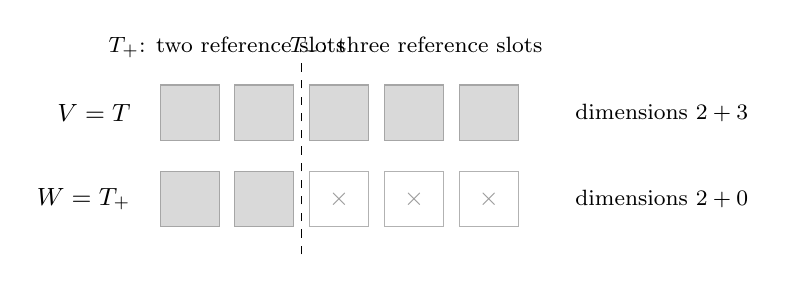
\begin{tikzpicture}[x=1cm,y=1cm,font=\small]
\node[anchor=east] at (-.25,1.65) {$V=T$};\node[anchor=east] at (-.25,.55) {$W=T_+$};
\foreach \j in {0,...,4}{\draw[fill=black!15,draw=black!35] (\j*.95,1.3) rectangle ++(.75,.7);}
\foreach \j in {0,1}{\draw[fill=black!15,draw=black!35] (\j*.95,.2) rectangle ++(.75,.7);}
\foreach \j in {2,3,4}{\draw[black!30] (\j*.95,.2) rectangle ++(.75,.7);\node[text=black!40] at (\j*.95+.375,.55) {$\times$};}
\draw[dashed] (1.80,-.15)--(1.80,2.35);
\node[font=\footnotesize] at (.85,2.48) {$T_+$: two reference slots};
\node[font=\footnotesize] at (3.25,2.48) {$T_-$: three reference slots};
\node[font=\footnotesize,anchor=west] at (5.15,1.65) {dimensions $2+3$};
\node[font=\footnotesize,anchor=west] at (5.15,.55) {dimensions $2+0$};
\end{tikzpicture}
\end{center}
\captiontext{Squares refer to the local bases of the regular module. Crossed reference slots are absent from $W$; they are not additional basis vectors of $W$.}

\begin{center}
\begin{tabular}{@{}lcc@{}}\toprule
 & regular module $V$ & first-factor module $W$\\\midrule
$\dim e_+(-)$ & 2 & 2\\
$\dim e_-(-)$ & 3 & 0\\
Support & both maximal points & only the $+$ point\\
Trace of $e_-$ & 3 & 0\\\bottomrule
\end{tabular}
\end{center}

\head{A generalized packet is not its residue-field fiber}
At the point $z=1$, the full local packet $e_+V$ has dimension two, but its scalar fiber is
\[
V\otimes_{T,\,z\mapsto1}\QQ
\cong T_+/(\varepsilon)\cong\QQ.
\]
The packet has the basis $1,\varepsilon$. Its scalar fiber kills $\varepsilon$. The ordinary eigenspace is instead the kernel of multiplication by $\varepsilon$, spanned by $\varepsilon$. In this example the last two spaces have the same dimension, but they are obtained by different operations.

For $W$, the fiber at $z=-1$ is zero. At $z=1$ it is nonzero. The field-fiber criterion detects exactly the support of the supplied module.

\takeaway{A ring factor describes an available packet location. A nonzero localized module certifies occupancy there. A field fiber then specializes that module; it is not the whole generalized packet.}

% ---------------------------------------------------------------------------
\vpage{14}{At two, division is the obstruction}{A COEFFICIENT-PRIME BOUNDARY}{Main text: Section 5, Remark 8.5 and Section 11}
Let $C_2=\langle g:g^2=1\rangle$. Over $\QQ_2$, the two familiar sign projectors are
\[
e_+=\frac{1+g}{2},\qquad e_-=\frac{1-g}{2},
\qquad \QQ_2[C_2]\cong\QQ_2\times\QQ_2.
\]
They do not belong to $\ZZ_2[C_2]$. Therefore one cannot first use them integrally and then reduce modulo two.

\head{Compute the actual residual algebra}
Over $\FF_2$, put $\delta=g-1=g+1$. Then $\delta^2=g^2-2g+1=0$ and
\[
\FF_2[C_2]\cong\FF_2[\delta]/(\delta^2).
\]
The two sign eigenvalues have merged. The ring is local and retains a nilpotent direction instead of two residual projector pieces.

\begin{minipage}[c]{.48\linewidth}
\centering
\begin{tabular}{@{}ccc@{}}\toprule
Element & Square & Idempotent?\\\midrule
$0$ & $0$ & yes\\
$1$ & $1$ & yes\\
$\delta$ & $0$ & no\\
$1+\delta$ & $1$ & no\\\bottomrule
\end{tabular}
\end{minipage}\hfill
\begin{minipage}[c]{.47\linewidth}
In the basis $1,\delta$, multiplication by $g=1+\delta$ is
\[
G=\begin{pmatrix}1&0\\1&1\end{pmatrix},\qquad
G^2=I\quad\text{over }\FF_2.
\]
It is not the identity: $G-I$ is nonzero and square-zero.
\end{minipage}

\head{A trace can vanish while a packet is occupied}
The identity projector on $\FF_2^2$ has rank two and trace $2=0$. Hence nonzero rank and nonzero trace are not equivalent in this characteristic. The localization and rank criteria still detect the nonzero space. The characteristic-zero qualification in Corollary 8.4 is essential.

\head{Recovery without averaging}
The augmentation map sends $g$ to $1$ and has kernel $(g-1)$. Thus
\[
\ZZ_2[C_2]/(g-1)\cong\ZZ_2,
\qquad
\bigl(\ZZ_2[C_2]^r\bigr)/(g-1)\ZZ_2[C_2]^r\cong\ZZ_2^r.
\]
These quotient identities require no division by two. They explain why augmentation and coinvariants remain usable even when sign-projector formulas do not.

\takeaway{Use the algebra available at the coefficient prime. Augmentation recovery is valid here; it still does not prove full deformation support or supply a universal automorphy theorem at two.}

% ---------------------------------------------------------------------------
\vpage{15}{Nonzero at every level is not enough}{INVERSE SYSTEMS / THE STABLE CORE}{Main text: Definition 8.9, Lemma 8.10 and Theorem 8.11}
Let every level be $V_m=k^3$. For a transition matrix $F$, compatibility means $v_m=Fv_{m+1}$. The directions visible at level $m$ after looking $h$ levels ahead form $\im(F^h)$.

\begin{minipage}[t]{.48\linewidth}\centering
{\sffamily\bfseries A surviving direction}\par
\[
P=\begin{pmatrix}1&0&0\\0&0&0\\0&0&0\end{pmatrix},\qquad P^2=P.
\]
\vfig[.45]{core_projection}
\captiontext{At every positive horizon, precisely the $e_1$ direction remains visible.}
\end{minipage}\hfill
\begin{minipage}[t]{.48\linewidth}\centering
{\sffamily\bfseries Every direction eventually dies}\par
\[
N=\begin{pmatrix}0&1&0\\0&0&1\\0&0&0\end{pmatrix},\qquad N^3=0.
\]
\vfig[.45]{core_nilpotent}
\captiontext{Image dimensions are $3,2,1,0,0,\ldots$, although every level still has dimension three.}
\end{minipage}

\head{Now compute the limits, not just their level dimensions}
For the $P$-system, the limit consists of the constant compatible sequences $(a e_1,a e_1,\ldots)$, so it is isomorphic to $k$. For the $N$-system, every compatible sequence satisfies
\[
v_m=N^3v_{m+3}=0\quad\text{for every }m,
\]
and the limit is zero. This is an all-level argument from the identity $N^3=0$, not a finite experimental guess.

\head{What the stable core measures}
In a general inverse system of finite-dimensional spaces,
\[
Y_m=\bigcap_{n\ge m}\im(f_{n,m})
\]
contains exactly the vectors visible from arbitrarily remote levels. The paper proves that the transition maps restrict to surjections $Y_{m+1}\twoheadrightarrow Y_m$. A prescribed nonzero vector in $Y_1$ can then be lifted recursively to a coherent nonzero sequence.

\takeaway{The stable core tests persistence through the transition maps. Counting nonzero spaces at separate levels does not test persistence.}

% ---------------------------------------------------------------------------
\vpage{16}{Finite dimension prevents tail escape}{TWO DIFFERENT COMPACTNESS MECHANISMS}{Main text: Theorem 8.7, Corollary 8.8 and Example 8.13}
Nested nonzero subspaces inside \emph{one fixed finite-dimensional space} behave differently from nested tails inside an infinite-dimensional space.

\begin{minipage}[t]{.44\linewidth}\centering
{\sffamily\bfseries Fixed carrier $k^5$}\par\vspace{4pt}
\vfig[.75]{nested_finite}
\captiontext{The projectors retain initial basis directions with dimensions $5,4,4,2,1,1,\ldots$. In this explicitly defined example the projector is constant from level five onward.}
\end{minipage}\hfill
\begin{minipage}[t]{.52\linewidth}\centering
{\sffamily\bfseries Infinite carrier $\ell^2(\mathbb N)$}\par\vspace{4pt}
\vfig[.91]{infinite_tail}
\captiontext{Row $m$ retains all basis vectors $e_j$ with $j\ge m$. Every row continues infinitely to the right. The display is a finite window, not a truncation of the actual carrier.}
\end{minipage}

\head{Why the finite chain eventually stops changing}
Suppose idempotents satisfy
\[
e_{m+1}e_m=e_me_{m+1}=e_{m+1}.
\]
Their ranges are nested. In dimension $d$, nonzero ranges allow at most $d-1$ strict dimension drops. There may be long gaps between drops, but only finitely many drops. The chain therefore becomes constant and has nonzero intersection.

\begin{insight}
A single repeated dimension does \emph{not} certify final stabilization. The finite example deliberately has a plateau $4,4$ before another drop. Finite dimension bounds the number of strict drops, not the time of the last one.
\end{insight}

\head{Why every infinite tail can be nonzero while their intersection vanishes}
Let $P_m$ project onto the closed span of $e_m,e_{m+1},\ldots$. Each range is nonzero. But a vector belonging to every range has its $j$-th coordinate zero once $m>j$. Every coordinate is therefore zero:
\[
\bigcap_{m\ge1}P_m\ell^2(\mathbb N)=\{0\}.
\]

\takeaway{Fixed finite-carrier stabilization, stable images in an inverse system, and infinite Hilbert-space tails are different situations. Their hypotheses cannot be exchanged.}

% ---------------------------------------------------------------------------
\vpage{17}{Where the arithmetic still enters}{THE CONDITIONAL THEOREM / INPUTS AND CONSEQUENCES}{Main text: revised Theorem 12.6 and Section 13}
The final theorem is a composition of proved implications with explicitly supplied data. These are not competing labels: an implication may be internally proved while its arithmetic premises remain external.

{\small
\begin{tabularx}{\linewidth}{@{}p{.13\linewidth}YY@{}}\toprule
\textbf{Gate} & \textbf{What must be supplied} & \textbf{What the formal deduction gives}\\\midrule
Residual & Residual automorphic occupancy and a represented deformation problem. & The rings, universal representation, and starting carrier are available as inputs.\\
Patching & An applicable patching package: full patched support, quotient, and control isomorphism. & Full support descends to the finite-level module or perfect complex.\\
Comparison & A ring map $f:R\to T$ with the stated support comparison, or the suitable isomorphism and carrier identification. & Support is transported at compatible points.\\
Fiber & A Hecke point $y:T\to E'$ over the same field, with $y\circ f=x$. & A nonzero scalar fiber and an actual eigensystem; in the derived case, one survives in a cohomological degree.\\
Realization & Classicality for that eigensystem, an attached representation, continuity, dense Frobenius comparison, and semisimplification/rigidity inputs. & The specialization is identified after semisimplification with the attached representation.\\\bottomrule
\end{tabularx}}

\head{Support alone does not supply a point over the same field}
The inclusion $\QQ\to\QQ(i)$ preserves full support of the nonzero scalar-extended carrier. But no $\QQ$-algebra map $\QQ(i)\to\QQ$ exists: the image of $i$ would be a rational number $a$ with $a^2=-1$. Thus one cannot infer the required Hecke point $y$ merely from a support statement.

\head{Propagation needs two existing families and the same automorphic object}
After producing an automorphic object $\pi$, retain \emph{that same} $\pi$. The propagation statement assumes both the original compatible family and the family attached to $\pi$ already exist, with the common Frobenius polynomial data and the stated comparison hypotheses. It then identifies corresponding members. It does not construct a missing family.

\takeaway{The algebra locates and transports supplied nonzero data. Arithmetic inputs establish occurrence, classicality, and attachment. A visualization must not turn one of those inputs into an automatic consequence.}

% ---------------------------------------------------------------------------
\vpage{18}{Return to the proofs with a concrete object}{READING ROUTE / SOURCE CROSSWALK / CHECKS}{Companion to the 36-page Paper XII manuscript, formal release v0.17.0}
Use the example on the left to keep the relevant object in view while reading the exact statement on the right. The appendix is explanatory; the main text supplies the theorem hypotheses and the proof contract.

{\small
\begin{tabularx}{\linewidth}{@{}p{.12\linewidth}Yp{.30\linewidth}@{}}\toprule
\textbf{Appendix} & \textbf{Question or calculation} & \textbf{Paper XII reference}\\\midrule
V--3 & Quotient monomials before or after completed combination & Theorem 3.1; Corollary 3.2\\
V--4 & A test point factors exactly when its local equations vanish & Proposition 3.3\\
V--5 & Compatible precision data and the closed-kernel argument & Section 3; Section 10\\
V--6--7 & Minors, fiber dimensions, support, and nilpotent structure & Theorems 6.3--6.4\\
V--8 & Base change and transport of intrinsic Fitting ideals & Proposition 6.5; Theorem 7.1\\
V--9 & A quotient loses a generic point without creating a projector & Propositions 3.4 and 7.3\\
V--10 & Auxiliary freeness versus full deformation support & Theorems 6.7, 6.9, 6.11; Example 6.13\\
V--11 & A two-term projective complex and its derived fibers & Definition 6.14; Theorem 6.16\\
V--12--13 & Whole primary packets, localization, and scalar fibers & Theorems 7.4, 8.2; Corollaries 8.3--8.4\\
V--14 & Sign-projector failure and augmentation recovery & Section 5; Remark 8.5; Section 11\\
V--15--16 & Stable images, finite stabilization, and tail escape & Section 8, items 8.7--8.13\\
V--17 & Compatible Hecke points and conditional realization & Theorem 12.6; Section 13\\\bottomrule
\end{tabularx}}

\head{Three short proof-reading tests}
\textbf{Can a module have full support but fail to be faithful?} Yes. On \pagerefV{10}, the module $k$ over $k[[x]]/(x^2)$ has a nonzero nilpotent annihilator and full support.

\textbf{Do equal support sets force equal Fitting ideals?} No. On \pagerefV{7}, $(xy)$ and $(x^2y)$ have the same vanishing set but different infinitesimal behavior.

\textbf{Do nonzero finite levels force a nonzero inverse limit?} No. On \pagerefV{15}, $N^3=0$ forces every compatible sequence to vanish, although every level is $k^3$.

\head{Provenance and reproducibility}
The source is \emph{Patching Support, Hecke Packets, and Conditional Automorphic Completion}, Komorebi P., revised formalization v0.17.0. The theorem references above are internal references to that manuscript. The existing 49-claim revised formal contract and its inherited original-wording boundaries are unchanged.

The accompanying Python script performs \textbf{31 exact checks}: exhaustive finite test-ring enumeration, symbolic minors and CRT identities, exact matrix calculations, and the identities behind the stable-core examples. All drawings are reproducible vector graphics. The new examples were not added to Lean and the Lean suite was not rerun for this editorial appendix. Infinite claims are supported by the arguments given here, not by extrapolating a finite image.

\end{document}
